\section{Phương pháp nghiên cứu và giải pháp đề xuất}
\label{sec:phuong_phap}

Nhằm hiện thực hóa nguyên lý phân tách trách nhiệm (Two-Stage Decoupling), hệ thống được cấu trúc thành một luồng xử lý tuần tự kết hợp rẽ nhánh mô-đun hóa cao độ. Hình~\ref{fig:detailed_pipeline_block} trực quan hóa chi tiết từng mắt xích xử lý, quy định chặt chẽ dữ liệu đầu vào và định dạng đầu ra của từng khối chức năng.

\begin{figure}[H]
\centering
\resizebox{\textwidth}{!}{%
\begin{tikzpicture}[
    node distance=0.9cm and 0.5cm,
    block/.style={rectangle, draw=deepgreen, fill=softgreen, thick, rounded corners=3pt, align=center, minimum height=1.2cm, inner sep=6pt, font=\small},
    branchA/.style={rectangle, draw=maingreen!90!black, fill=cream, thick, rounded corners=3pt, align=center, minimum height=1.1cm, inner sep=5pt, font=\small},
    branchB/.style={rectangle, draw=blue!70!black, fill=blue!5, thick, rounded corners=3pt, align=center, minimum height=1.1cm, inner sep=5pt, font=\small},
    line/.style={draw=deepgreen, ->, >=stealth, thick},
    font=\small
]
    \node [block] (input) {\textbf{Đầu vào Toàn cảnh}\\Ảnh RGB\\$960\times 540$ / $1920\times 1080$};
    
    \node [block, right=of input] (m1) {\textbf{Mô-đun M1: YOLO11s 1-Class}\\Vào: Ảnh kích thước $\text{imgsz}=800$\\Ra: Danh sách tọa độ hộp bao\\$(x_1, y_1, x_2, y_2, \text{conf})$, $\text{conf} \ge 0.25$};
    
    \node [block, right=of m1] (m2) {\textbf{Mô-đun M2: Cắt ROI}\\Vào: Ảnh gốc + Bounding boxes\\Xử lý: Trích xuất ảnh con (Crop)\\\& Lưu tỷ lệ khung hình gốc $\text{AR}$\\Ra: Crop RGB + $W_{\text{orig}}/H_{\text{orig}}$};
    
    \node [branchA, above right=0.35cm and 0.7cm of m2] (m3a) {\textbf{Mô-đun M3A: Thị giác Truyền thống}\\Vào: Crop ROI + Tỷ lệ $\text{AR}$\\Xử lý: Chuỗi đặc trưng $S0 \rightarrow S3$\\Vector đa chiều $\mathbb{R}^{457} \rightarrow$ SVM (RBF)\\Ra: Nhãn nhóm quy chuẩn (0..3)};
    
    \node [branchB, below right=0.35cm and 0.7cm of m2] (m3b) {\textbf{Mô-đun M3B: Học sâu Hiện đại}\\Vào: Crop ROI chuẩn hóa $64\times 64$\\Xử lý: Enhanced LeNet-5 (PyTorch)\\Khối ConvBlock 1..3 + Classifier\\Ra: Nhãn nhóm quy chuẩn (Softmax)};
    
    \node [block, right=5.2cm of m2] (output) {\textbf{Đầu ra Hệ thống}\\Ảnh toàn cảnh gắn nhãn\\Hộp bao định vị + Mã màu nhóm\\\& Thống kê độ trễ toàn trình};

    \path [line] (input) -- (m1);
    \path [line] (m1) -- (m2);
    \path [line] (m2.east) |- node[above, pos=0.7, font=\scriptsize] {Nhánh A} (m3a.west);
    \path [line] (m2.east) |- node[below, pos=0.7, font=\scriptsize] {Nhánh B} (m3b.west);
    \path [line] (m3a.east) -| (output.north);
    \path [line] (m3b.east) -| (output.south);
\end{tikzpicture}%
}
\caption{Sơ đồ phân rã kỹ thuật chi tiết các mô-đun trong pipeline Two-Stage Hybrid Traffic Sign Recognition.}
\label{fig:detailed_pipeline_block}
\end{figure}
\vspace{-0.2cm}
\begin{quote}
\small \textbf{Đọc Hình~\ref{fig:detailed_pipeline_block}:} Sơ đồ thể hiện luồng xử lý khép kín từ ảnh camera hành trình qua bộ định vị đơn lớp M1, khâu trích xuất ảnh con M2, rẽ song song vào hai nhánh phân loại độc lập M3A (Thị giác truyền thống) và M3B (Học sâu), trước khi tích hợp kết quả cuối cùng lên khung hình.
\end{quote}

Bảng~\ref{tab:module_io_spec} tổng hợp đặc tả giao tiếp kỹ thuật giữa các mô-đun chức năng:

\begin{table}[H]
\centering
\small
\caption{Đặc tả giao tiếp đầu vào/đầu ra và phân công trách nhiệm từng mô-đun.}
\label{tab:module_io_spec}
\begin{tabularx}{\textwidth}{|c|p{3.2cm}|p{3.8cm}|p{3.2cm}|Y|}
\hline
\textbf{Mô-đun} & \textbf{Dữ liệu đầu vào} & \textbf{Xử lý kỹ thuật chính} & \textbf{Dữ liệu đầu ra} & \textbf{Thực hiện} \\
\hline
\textbf{M1} & Ảnh đường phố RGB ($960\times 540$ hoặc $1920\times 1080$) & Suy luận YOLO11s chuyên biệt 1-lớp (\texttt{sign}), lọc ngưỡng $\text{conf} \ge 0.25$, áp dụng NMS IoU $0.6$ & Danh sách tọa độ $K$ hộp bao $(x_1, y_1, x_2, y_2, \text{conf})$ & Từ Lê Tuấn Anh \\
\hline
\textbf{M2} & Khung hình ảnh gốc + Danh sách hộp bao từ M1 & Cắt ma trận pixel con (ROI crop), đo đạc và lưu trữ tỷ lệ khung hình thực tế $\text{AR} = W/H$ trước khi resize & Tập hợp các ảnh con $\mathbf{I}^{(k)}_{\text{crop}}$ kèm giá trị $\text{AR}_k$ ban đầu & Từ Lê Tuấn Anh \\
\hline
\textbf{M3A} & Ảnh con ROI crop + Tỷ lệ khung hình $\text{AR}$ & Dịch pha Hue, tính histogram HSV cục bộ 2x2, trích xuất HOG trên ảnh xám $\rightarrow$ Vector 457 chiều $\rightarrow$ SVM RBF & Nhãn dự đoán thuộc 4 nhóm QCVN và xác suất tin cậy & Từ Lê Tuấn Anh \\
\hline
\textbf{M3B} & Ảnh con ROI crop được resize về $64\times 64\times 3$ & Chuẩn hóa ImageNet, lan truyền thuận qua Enhanced LeNet-5 gồm 3 khối Conv-BN-ReLU-Pool và 2 tầng Dropout & Phân phối xác suất Softmax trên 4 nhóm quy chuẩn & Nguyễn Thanh Tân \\
\hline
\end{tabularx}
\end{table}

\subsection{Giai đoạn 1: Mô-đun phát hiện YOLO11s (1-Class Detector) -- Từ Lê Tuấn Anh}
\label{subsec:stage1_yolo}

\subsubsection{Lý do thiết kế Detector chuyên biệt đơn lớp (1-Class "sign")}
\label{subsubsec:why_one_class}

Trong các nghiên cứu nhận dạng biển báo truyền thống sử dụng mô hình One-Stage đa lớp (chẳng hạn gán trực tiếp 52 lớp chi tiết hoặc 4 nhóm chức năng ngay tại tầng phát hiện của mạng tích chập), bộ phát hiện luôn phải gánh chịu sự quá tải dung lượng biểu diễn (representation capacity overload). Nguyên nhân cốt lõi bao gồm:

\begin{enumerate}
    \item \textbf{Mâu thuẫn tỷ lệ kích thước vật thể:} Trên cùng một khung hình toàn cảnh góc rộng, các biển báo cự ly xa chỉ chiếm từ $8 \times 8\text{ px}$ đến $20 \times 20\text{ px}$ (chưa đầy $0.05\%$ diện tích canvas), trong khi bối cảnh nền đô thị chiếm tới $99.95\%$. Nếu bắt mạng nơ-ron phải đồng thời phân giải các hoa văn nội tại tinh xảo (như phân biệt hình mũi tên rẽ hay vạch cấm), trường tiếp nhận sâu ở tầng cao sẽ làm nhòe và tiêu biến tín hiệu biên cạnh của các biển báo nhỏ.
    \item \textbf{Tối ưu hóa độ phủ (Detection Recall):} Trong các hệ thống trợ lái xe ADAS, lỗi bỏ sót biển báo (False Negative) nguy hiểm hơn rất nhiều so với lỗi phát hiện nhầm một vùng nền (False Positive) vì các vùng nhầm lẫn có thể được bộ phân loại Tầng 2 loại bỏ tiếp theo. Việc quy đổi toàn bộ các lớp về nhãn nhị phân duy nhất \texttt{sign} cho phép $100\%$ trọng số mạng tập trung tối đa vào việc phân tách biên giới giữa "biển báo" và "hậu cảnh", từ đó tối đa hóa tỷ lệ bắt trúng ($\text{Recall} = 85.61\%$).
\end{enumerate}

\subsubsection{Dữ liệu tiền huấn luyện CCTSDB và dữ liệu Việt Nam}
\label{subsubsec:pretrain_cctsdb_vn}

Để bảo đảm tính thích ứng cao và khả năng tổng quát hóa vượt trội, mô hình được xây dựng qua quy trình xử lý dữ liệu chuẩn hóa nghiêm ngặt:

\begin{itemize}
    \item \textbf{Tập dữ liệu tiền huấn luyện CCTSDB 2021 (China City Traffic Sign Database):}
    \begin{itemize}
        \item Gồm 17.856 ảnh có nhãn ban đầu thuộc 3 nhóm biển báo (`prohibitory`, `mandatory`, `warning`). Nhóm thực hiện ánh xạ đồng nhất toàn bộ 3 nhóm về nhãn đơn lớp \texttt{sign} (Class ID 0).
        \item Bổ sung \textbf{500 ảnh âm tính (Negative Images)} chứa cảnh quan đường sá, cây cối, nhà cửa và biển quảng cáo thương mại nhưng tuyệt đối không chứa biển báo giao thông. Toàn bộ 500 ảnh này được đổi tên chuẩn hóa theo định dạng stem thống nhất và gán tệp nhãn rỗng (0-byte text file). Bước này mang ý nghĩa sống còn giúp mạng học cách dập tắt các phản ứng kích hoạt sai trên các kết cấu nền phức tạp.
        \item Tập validation của CCTSDB được tách biệt hoàn toàn theo các đoạn khối frame video liên tục nhằm ngăn chặn rò rỉ hình thái học.
    \end{itemize}

    \item \textbf{Tập dữ liệu biển báo giao thông Việt Nam:}
    \begin{itemize}
        \item Gồm 3.216 ảnh chụp thực tế ngoài đường phố Việt Nam ở hai độ phân giải phổ biến ($960 \times 540$ chiếm $73.5\%$ và $1920 \times 1080$ chiếm $25.2\%$).
        \item Toàn bộ 52 mã hiệu biển báo chi tiết theo QCVN 41:2019 được ánh xạ gộp về nhãn 1-lớp \texttt{sign}.
        \item Áp dụng triệt để thuật toán \textbf{Block Split} (chia khối 100 frame liên tục kết hợp khoảng đệm 5 frame an toàn) tạo ra 3 tập dữ liệu độc lập: Train (2.215 ảnh / 16.203 bbox ban đầu), Val (270 ảnh / 568 bbox) và Test (550 ảnh / 1.845 bbox).
    \end{itemize}
\end{itemize}

\begin{figure}[H]
\centering
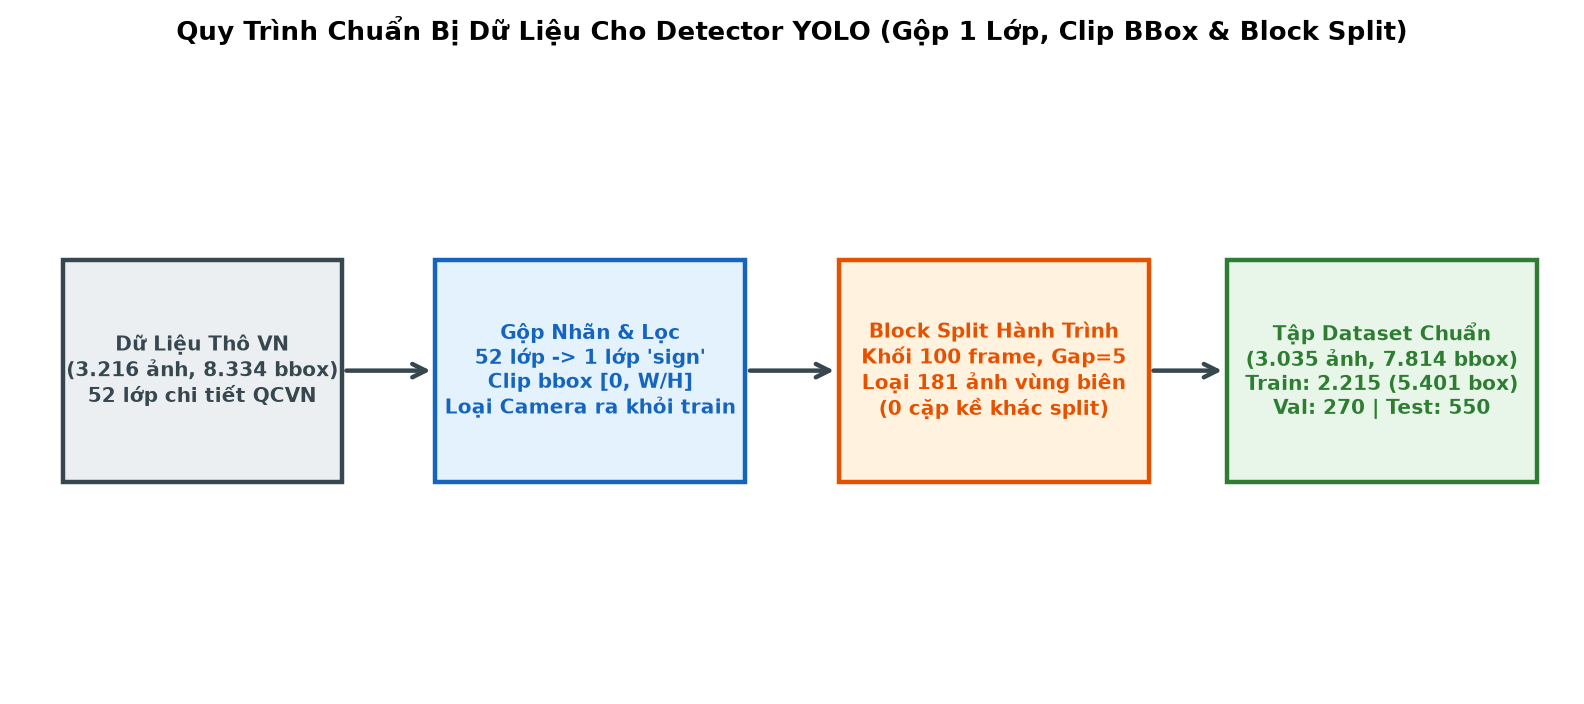
\includegraphics[width=0.88\textwidth]{graphics/sec3/f2_04_data_prep_flowchart.png}
\caption{Quy trình tiền xử lý, gộp nhãn đơn lớp và bổ sung ảnh âm tính cho bộ dữ liệu CCTSDB và Việt Nam.}
\label{fig:data_prep_flowchart}
\end{figure}
\vspace{-0.2cm}
\begin{quote}
\small \textbf{Đọc Hình~\ref{fig:data_prep_flowchart}:} Sơ đồ thể hiện quy trình hợp nhất nhãn từ 3 lớp CCTSDB và 52 lớp Việt Nam về nhãn duy nhất \texttt{sign}, tích hợp 500 mẫu nền âm tính và phân chia Block Split nhằm triệt tiêu hoàn toàn rò rỉ dữ liệu.
\end{quote}

\subsubsection{Chuỗi chuyển giao học tập hai giai đoạn (Two-Stage Transfer Learning)}
\label{subsubsec:transfer_learning_chain}

Quá trình chuyển giao trọng số được mô hình hóa theo chuỗi liên tục: Khởi tạo từ trọng số tổng quát \textbf{COCO} $\xrightarrow{\text{Pretrain}}$ Tập miền tương đồng \textbf{CCTSDB} $\xrightarrow{\text{Fine-tune}}$ Miền mục tiêu \textbf{Việt Nam}.

\begin{figure}[H]
\centering
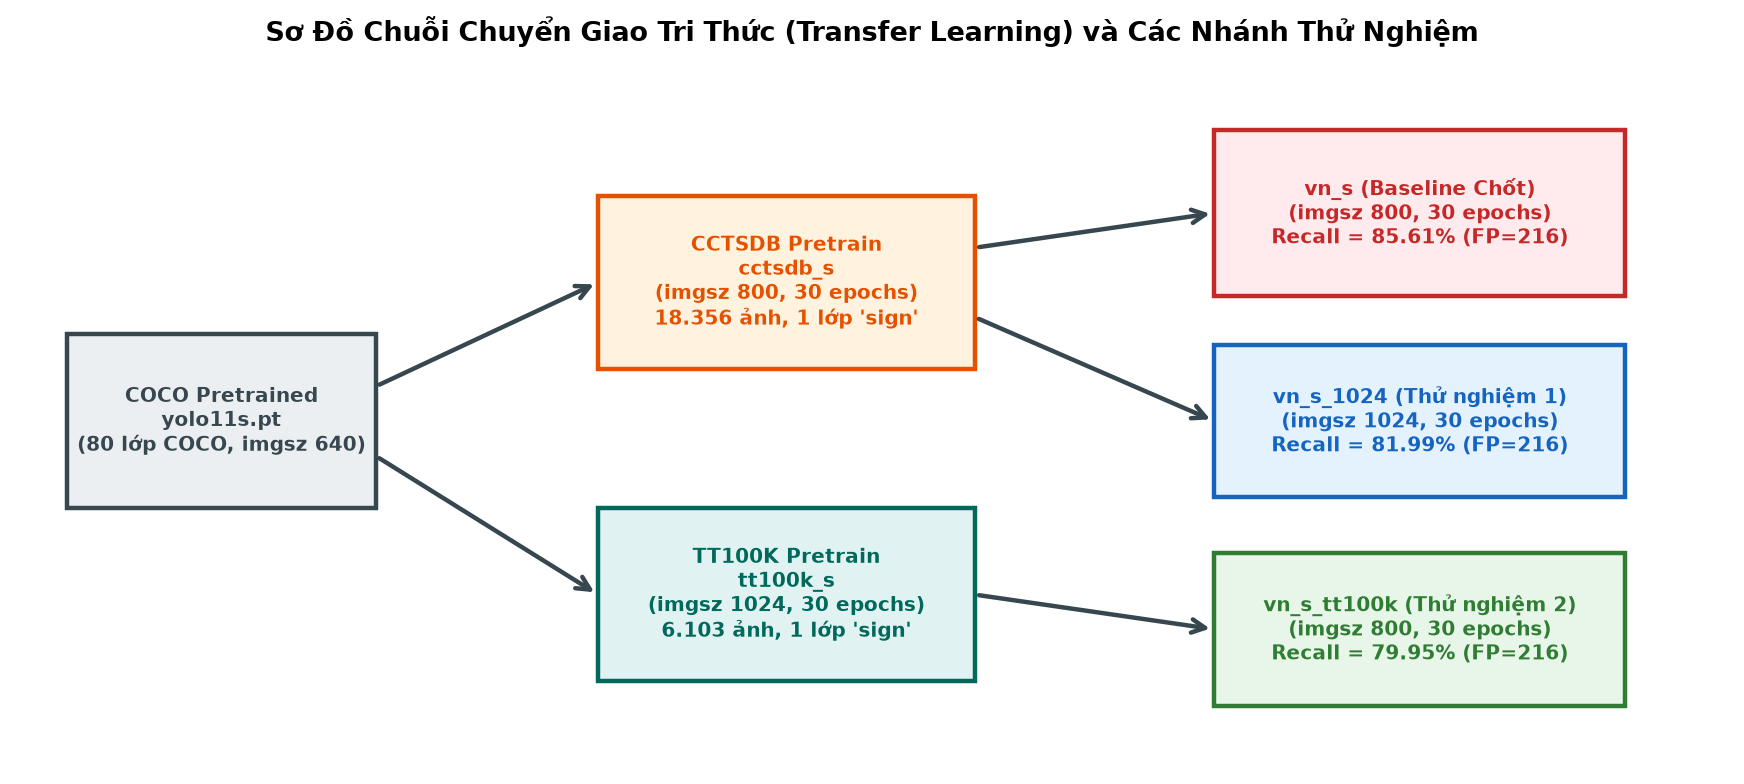
\includegraphics[width=0.92\textwidth]{graphics/sec3/f2_01_transfer_learning_chain.png}
\caption{Sơ đồ chuỗi chuyển giao tri thức hai giai đoạn từ COCO qua CCTSDB đến tập dữ liệu Việt Nam.}
\label{fig:transfer_learning_chain}
\end{figure}
\vspace{-0.2cm}
\begin{quote}
\small \textbf{Đọc Hình~\ref{fig:transfer_learning_chain}:} Mũi tên 1 thể hiện giai đoạn tiền huấn luyện trên 17.856 ảnh CCTSDB ở kích thước $\text{imgsz}=800$ qua 30 epochs; Mũi tên 2 thể hiện giai đoạn tinh chỉnh trên dữ liệu Việt Nam ở cùng kích thước $\text{imgsz}=800$ qua 30 epochs, kế thừa toàn bộ tri thức biểu diễn biên cạnh từ CCTSDB.
\end{quote}

\subsubsection{Bảng cấu hình siêu tham số huấn luyện (Trích xuất từ \texttt{args.yaml})}
\label{subsubsec:yolo_hyperparams}

Để đảm bảo tính minh bạch khoa học tuyệt đối, toàn bộ siêu tham số của các tiến trình huấn luyện được trích xuất trực tiếp từ các tệp \texttt{args.yaml} trong thư mục lưu trữ thực nghiệm, hoàn toàn không phỏng đoán. Bảng~\ref{tab:yolo_training_configs} tổng hợp chi tiết cấu hình của 4 mô hình:

\begin{table}[H]
\centering
\small
\caption{Bảng cấu hình siêu tham số và thời gian huấn luyện thực nghiệm của các mô hình YOLO (trích xuất từ \texttt{args.yaml}).}
\label{tab:yolo_training_configs}
\begin{tabularx}{\textwidth}{|p{3.8cm}|p{2.8cm}|p{2.8cm}|p{2.8cm}|Y|}
\hline
\textbf{Siêu tham số / Cấu hình} & \textbf{\texttt{cctsdb\_s} (Pretrain)} & \textbf{\texttt{vn\_s} (Baseline)} & \textbf{\texttt{vn\_s\_1024} (Thử nghiệm 1)} & \textbf{\texttt{vn\_s\_tt100k} (Thử nghiệm 2)} \\
\hline
Trọng số khởi tạo & \texttt{yolo11s.pt} (COCO) & \texttt{cctsdb\_s/best.pt} & \texttt{cctsdb\_s/best.pt} & \texttt{tt100k\_s/best.pt} \\
\hline
Tập dữ liệu huấn luyện & CCTSDB 2021 & Việt Nam (Train) & Việt Nam (Train) & Việt Nam (Train) \\
\hline
Kích thước canvas (\texttt{imgsz}) & \textbf{800} & \textbf{800} & \textbf{1024} & \textbf{800} \\
\hline
Số lượng Epochs & 30 & 30 & 30 & 30 \\
\hline
Kích thước lô (\texttt{batch}) & 4 & 4 & 4 & 4 \\
\hline
Số luồng dữ liệu (\texttt{workers}) & 0 & 0 & 0 & 0 \\
\hline
Độ chính xác hỗn hợp (\texttt{amp}) & True (FP16) & True (FP16) & True (FP16) & True (FP16) \\
\hline
Hạt ngẫu nhiên (\texttt{seed}) & 0 & 0 & 0 & 0 \\
\hline
Thuật toán tối ưu (\texttt{optimizer}) & \texttt{auto} (SGD/AdamW) & \texttt{auto} & \texttt{auto} & \texttt{auto} \\
\hline
Tốc độ học ban đầu (\texttt{lr0} / \texttt{lrf}) & 0.01 / 0.01 & 0.01 / 0.01 & 0.01 / 0.01 & 0.01 / 0.01 \\
\hline
Thiết bị thực thi (\texttt{device}) & NVIDIA RTX 4060 & NVIDIA RTX 4060 & NVIDIA RTX 4060 & NVIDIA RTX 4060 \\
\hline
\textbf{Thời gian huấn luyện đo được} & \textbf{17.410s ($\approx$ 4h 50m)} & \textbf{2.468s ($\approx$ 41m 08s)} & \textbf{3.568s ($\approx$ 59m 28s)} & \textbf{2.492s ($\approx$ 41m 32s)} \\
\hline
\end{tabularx}
\end{table}

\subsubsection{Hàm mất mát huấn luyện (Task-Aligned Loss)}
\label{subsubsec:yolo_loss_formula}

Mô hình duy trì cấu trúc hàm mất mát Task-Aligned Loss nguyên bản của YOLO11s gồm 3 thành phần liên kết chặt chẽ:
\begin{equation}
    \mathcal{L}_{\text{total}} = \lambda_{\text{box}} \mathcal{L}_{\text{CIoU}} + \lambda_{\text{dfl}} \mathcal{L}_{\text{DFL}} + \lambda_{\text{cls}} \mathcal{L}_{\text{BCE}}
    \label{eq:yolo_task_aligned_loss}
\end{equation}
với các trọng số cân bằng chuẩn $\lambda_{\text{box}} = 7.5$, $\lambda_{\text{dfl}} = 1.5$, và $\lambda_{\text{cls}} = 0.5$:
\begin{itemize}
    \item $\mathcal{L}_{\text{CIoU}}$: Đo lường độ trùng khớp hình học hộp bao, phạt khoảng cách tâm Euclidean và sự sai lệch tỷ lệ khung hình giữa hộp dự đoán và nhãn gốc.
    \item $\mathcal{L}_{\text{DFL}}$ (Distribution Focal Loss): Hồi quy các tọa độ biên dưới dạng phân phối xác suất liên tục quanh giá trị nhãn thực, giúp định vị sắc nét các cạnh biển báo bị mờ do chuyển động.
    \item $\mathcal{L}_{\text{BCE}}$ (Binary Cross-Entropy): Đo mất mát phân loại nhị phân cho sự hiện diện của biển báo đối với các anchor được gán nhãn tích cực.
\end{itemize}

\subsection{Giai đoạn 2A: Thị giác truyền thống (Color + Grid + HOG + SVM) -- Từ Lê Tuấn Anh}
\label{subsec:stage2_svm}

Trên mỗi ảnh con ROI được cắt ra từ các hộp bao của Tầng 1, phương pháp thị giác truyền thống xây dựng chuỗi trích xuất đặc trưng toán học đa nấc $S0 \rightarrow S3$ nhằm nắm bắt toàn diện từ phân bố màu sắc toàn cục, hình thái học không gian đến kết cấu biên cạnh định hướng.

\subsubsection{Chi tiết các nấc trích xuất đặc trưng \texorpdfstring{$S0 \rightarrow S3$}{S0 -> S3}}
\label{subsubsec:feature_steps_s0_s3}

\begin{enumerate}
    \item \textbf{Nấc S0 -- Phân bố màu sắc toàn cục HSV dịch pha vòng tròn (44 chiều):}
    \begin{itemize}
        \item \textit{Đầu vào:} Ảnh con ROI cắt từ ảnh gốc, co giãn về kích thước chuẩn hóa $32 \times 32\text{ px}$ theo chuẩn màu BGR.
        \item \textit{Thao tác kỹ thuật:} Chuyển đổi không gian màu sang HSV (\texttt{cv2.COLOR\_BGR2HSV}). Thực hiện phép dịch pha vòng tròn trên kênh Hue (dải giá trị $[0, 180)$ trong OpenCV):
        \begin{equation}
            H_{\text{shifted}} = (H + 30) \pmod{180}
            \label{eq:hue_circular_shift}
        \end{equation}
        Sau đó loại bỏ hoàn toàn kênh $V$ (Value), trích xuất biểu đồ 36 bins cho kênh $H_{\text{shifted}}$ và 8 bins cho kênh $S$ (Saturation), ghép nối và chuẩn hóa chuẩn $L_1$:
        \begin{equation}
            \mathbf{s}_0 = [\mathbf{h}_H, \mathbf{h}_S] \in \mathbb{R}^{36 + 8 = 44}, \quad \mathbf{s}_0 \leftarrow \frac{\mathbf{s}_0}{\sum \mathbf{s}_0 + \epsilon}
        \end{equation}
        \item \textit{Lý do toán học \& vật lý:} Kênh Hue mang bản chất topo vòng tròn ($0^\circ \equiv 180^\circ$). Màu đỏ đặc trưng của Biển Cấm và Biển Nguy Hiểm bị xẻ đôi ở hai đầu trục ($[0, 10]$ và $[170, 180]$). Phép dịch pha $+30^\circ$ đưa toàn bộ phổ màu đỏ về dải đơn liên tục $[30, 50]$, giúp histogram gom đỉnh năng lượng tập trung. Việc loại bỏ kênh $V$ giúp vector miễn nhiễm trước hiện tượng lóa nắng nhiệt đới, bóng râm che cắt mặt biển và điều kiện thiếu sáng.
    \end{itemize}

    \begin{figure}[H]
    \centering
    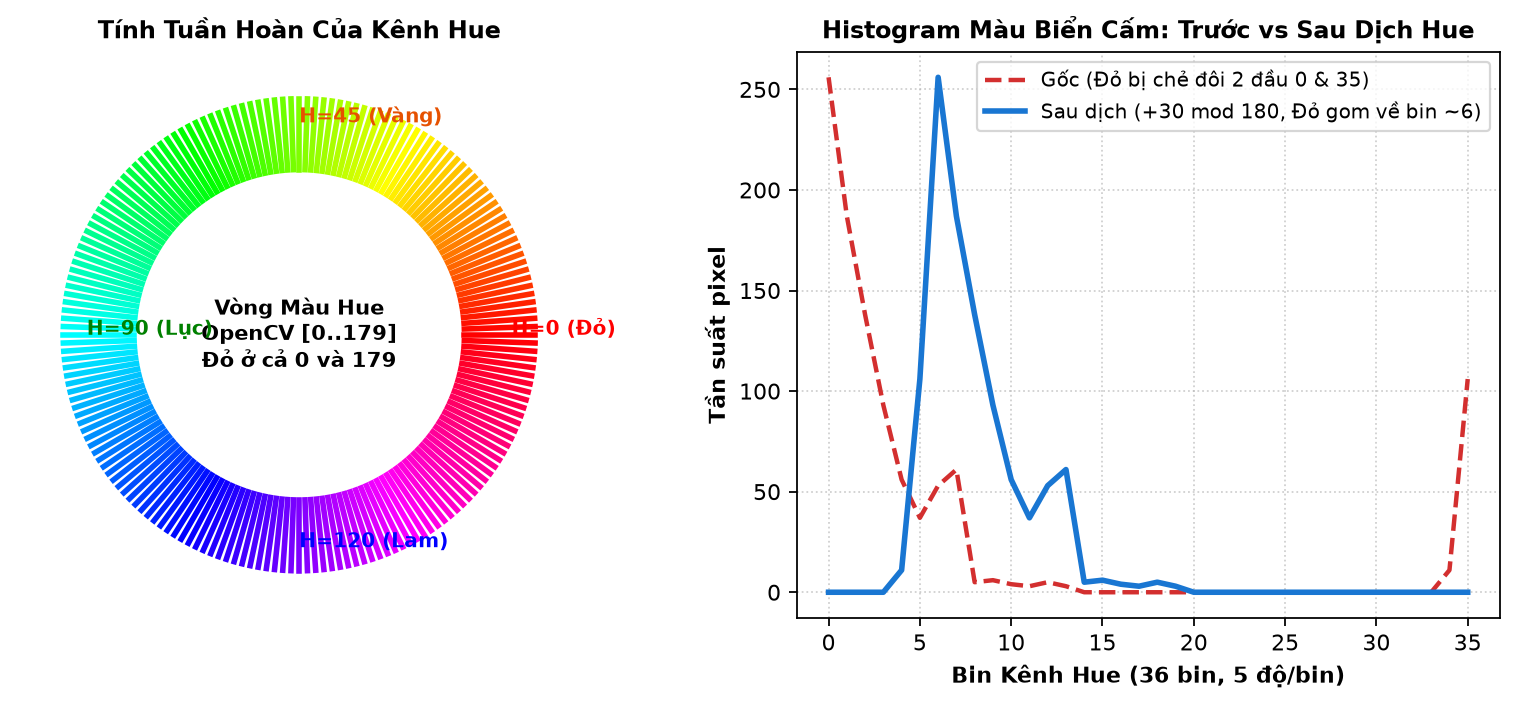
\includegraphics[width=0.88\textwidth]{graphics/sec3/f1_07_hue_circularity_shift.png}
    \caption{Trực quan hóa phép dịch pha vòng tròn kênh Hue ($+30^\circ$) giúp gom cụm màu đỏ liên tục.}
    \label{fig:hue_shift_demo}
    \end{figure}
    \vspace{-0.2cm}
    \begin{quote}
    \small \textbf{Đọc Hình~\ref{fig:hue_shift_demo}:} Biểu đồ bên trái cho thấy phân bố màu đỏ bị phân mảnh ở hai cực của dải Hue gốc; biểu đồ bên phải minh chứng sau phép biến đổi $(H+30)\%180$, toàn bộ tín hiệu màu đỏ được hội tụ trọn vẹn vào một đỉnh phân phối duy nhất.
    \end{quote}

    \item \textbf{Nấc S1 -- Tỷ lệ khung hình hình học ban đầu (45 chiều):}
    \begin{itemize}
        \item \textit{Đầu vào:} Vector đặc trưng $\mathbf{s}_0$ kết hợp tọa độ hộp bao ban đầu $(x_1, y_1, x_2, y_2)$ trên ảnh toàn cảnh.
        \item \textit{Thao tác kỹ thuật:} Tính tỷ lệ khung hình hình học ban đầu $\text{AR} = W_{\text{orig}} / H_{\text{orig}}$ \textbf{TRƯỚC KHI THỰC HIỆN RESIZE} ảnh con:
        \begin{equation}
            \mathbf{s}_1 = [\mathbf{s}_0, \text{AR}] \in \mathbb{R}^{44 + 1 = 45}
        \end{equation}
        \item \textit{Lý do kỹ thuật:} Nếu đo tỷ lệ sau khi co giãn ảnh con về $32 \times 32\text{ px}$, tỷ lệ $W/H$ luôn bị ép bằng $1.0$, làm mất sạch tín hiệu hình học. Trong thực tế, Biển Chỉ Dẫn thường có dạng chữ nhật nằm ngang ($\text{AR} > 1.2$), trong khi Biển Cấm và Biển Hiệu Lệnh là hình tròn ($\text{AR} \approx 1.0$), cung cấp thông tin phân định hình học quan trọng.
    \end{itemize}

    \item \textbf{Nấc S2 -- Lưới không gian Spatial Grid $2 \times 2$ (133 chiều):}
    \begin{itemize}
        \item \textit{Đầu vào:} Ảnh con kích thước $32 \times 32\text{ px}$ trong không gian màu HSV đã dịch pha.
        \item \textit{Thao tác kỹ thuật:} Chia đều ảnh con thành lưới $2 \times 2$ gồm 4 ô vuông cục bộ kích thước $16 \times 16\text{ px}$. Tại mỗi ô con $(i, j)$, trích xuất biểu đồ màu cục bộ rút gọn gồm 18 bins kênh $H$ và 4 bins kênh $S$ ($22\text{ chiều/ô}$):
        \begin{equation}
            \mathbf{s}_2 = [\mathbf{s}_1, \mathbf{c}_{11}, \mathbf{c}_{12}, \mathbf{c}_{21}, \mathbf{c}_{22}] \in \mathbb{R}^{45 + 4 \times 22 = 133}
        \end{equation}
        \item \textit{Lý do kỹ thuật:} Histogram toàn cục của S0 không chứa thông tin vị trí không gian. Lưới $2 \times 2$ giúp mô hình nắm bắt quy luật bố cục: Biển Cấm có viền đỏ ở 4 góc ô biên và màu trắng ở tâm; Biển Nguy Hiểm có viền đỏ bao quanh nền vàng trung tâm.
    \end{itemize}

    \begin{figure}[H]
    \centering
    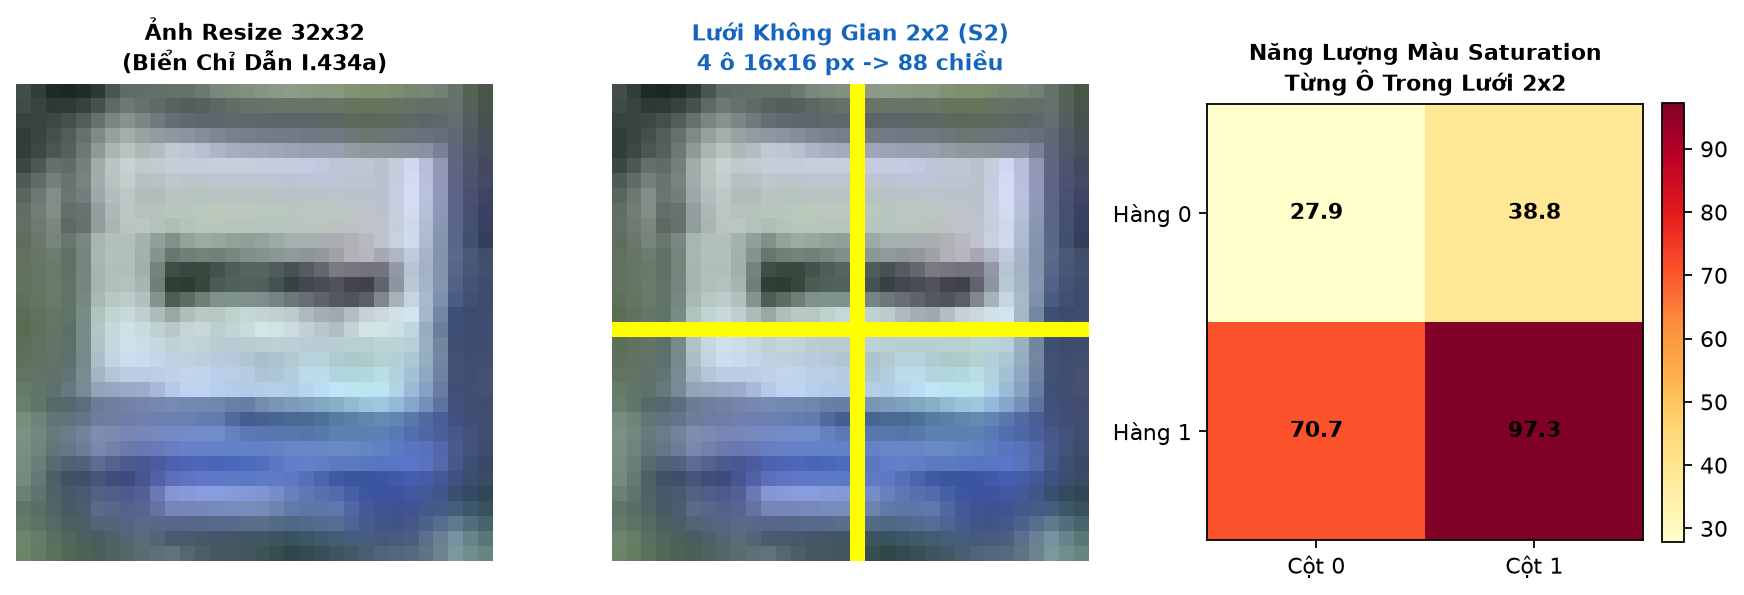
\includegraphics[width=0.75\textwidth]{graphics/sec3/f1_11_spatial_grid_heatmap.png}
    \caption{Bản đồ nhiệt phân bố màu sắc cục bộ qua lưới không gian Spatial Grid $2 \times 2$.}
    \label{fig:spatial_grid_heatmap}
    \end{figure}
    \vspace{-0.2cm}
    \begin{quote}
    \small \textbf{Đọc Hình~\ref{fig:spatial_grid_heatmap}:} Lưới không gian chia ảnh con thành 4 ô con độc lập, cho phép bóc tách cấu trúc viền ngoài và nền trong của các nhóm biển báo có bố cục hình học đối xứng.
    \end{quote}

    \item \textbf{Nấc S3 -- Gradient Định Hướng HOG trên ảnh xám (457 chiều -- Toàn diện nhất):}
    \begin{itemize}
        \item \textit{Đầu vào:} Ảnh con ROI co giãn về kích thước chuẩn hóa $64 \times 64\text{ px}$.
        \item \textit{Thao tác kỹ thuật (Xác nhận trực tiếp từ mã nguồn):} Chuyển đổi ảnh con sang \textbf{ẢNH XÁM (Grayscale)} bằng hàm \texttt{cv2.cvtColor(c64, cv2.COLOR\_BGR2GRAY)}, hoàn toàn không tính trên từng kênh màu riêng biệt. Áp dụng thuật toán \texttt{skimage.feature.hog} với các tham số:
        \begin{itemize}
            \item Kích thước ô (Pixels per cell): $16 \times 16\text{ px}$.
            \item Số hướng gradient (Orientations): 9 bins trên góc $[0^\circ, 180^\circ)$.
            \item Kích thước khối chuẩn hóa (Cells per block): $2 \times 2\text{ cells}$ ($32 \times 32\text{ px}$), bước trượt block stride: 1 cell ($16\text{ px}$).
            \item Số khối trên ảnh $64 \times 64$: $(\frac{64 - 32}{16} + 1) \times (\frac{64 - 32}{16} + 1) = 3 \times 3 = 9\text{ blocks}$.
            \item Số chiều HOG: $9 \text{ blocks} \times (2 \times 2 \times 9) = 9 \times 36 = \mathbf{324\text{ chiều}}$.
        \end{itemize}
        Vector đặc trưng đầy đủ của tầng S3 đạt:
        \begin{equation}
            \mathbf{s}_3 = [\mathbf{s}_2, \mathbf{h}_{\text{HOG}}] \in \mathbb{R}^{133 + 324 = \mathbf{457\text{ chiều}}}
            \label{eq:s3_full_vector}
        \end{equation}
        \item \textit{Lý do kỹ thuật:} Nấc đặc trưng cốt lõi giải quyết sự bế tắc của các mô hình dựa trên màu sắc khi đối mặt với cặp "Biển Hiệu Lệnh (xanh tròn)" và "Biển Chỉ Dẫn (xanh vuông/chữ nhật)". Vì hai nhóm này có phân bố histogram HSV giống hệt nhau, HOG trên ảnh xám nắm bắt chính xác góc định hướng tiếp tuyến của đường viền tròn cong đối lập với các góc vuông $90^\circ$ thẳng đứng.
    \end{itemize}

    \begin{figure}[H]
    \centering
    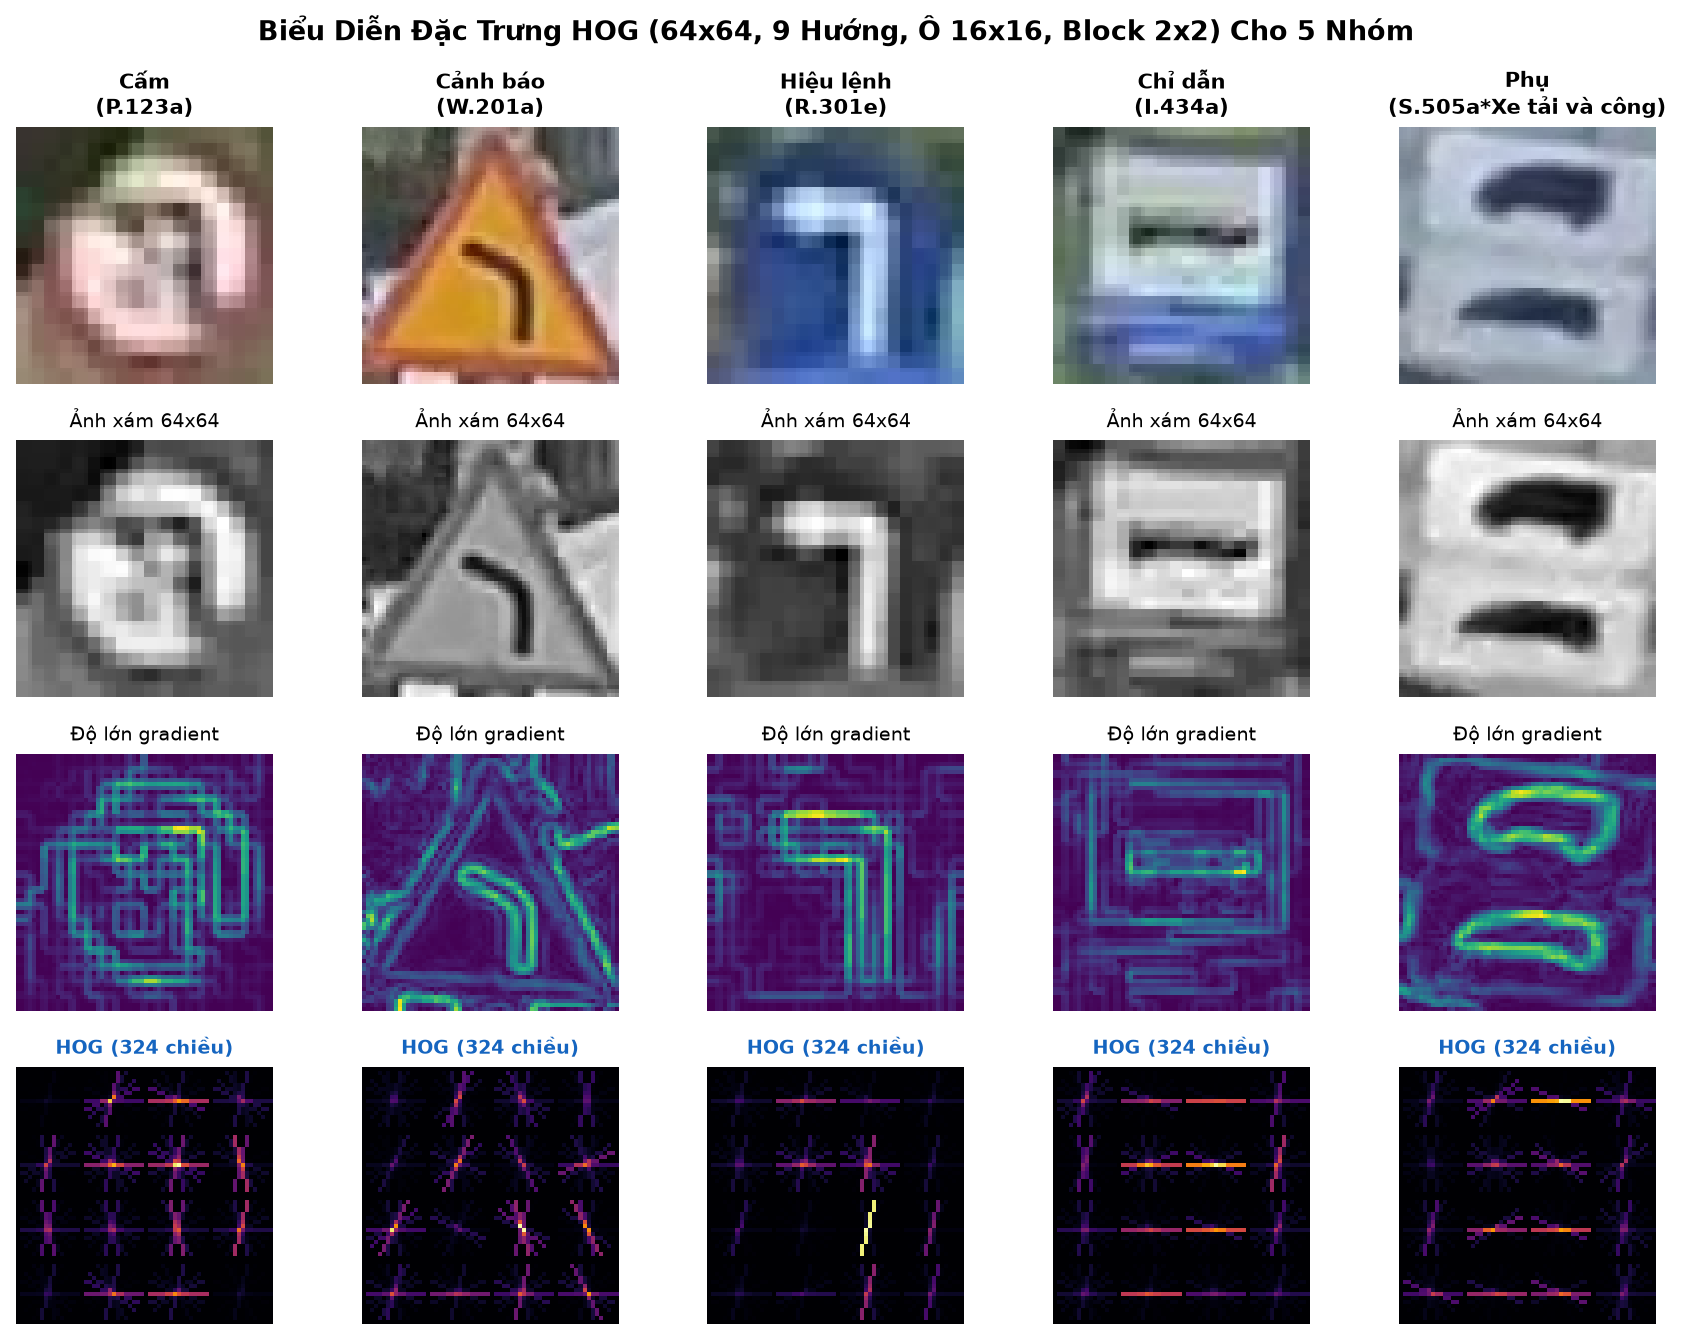
\includegraphics[width=0.88\textwidth]{graphics/sec3/f1_12_hog_visualization_groups.png}
    \caption{Trực quan hóa vector gradient định hướng HOG trên 4 nhóm biển báo mục tiêu.}
    \label{fig:hog_vis_groups}
    \end{figure}
    \vspace{-0.2cm}
    \begin{quote}
    \small \textbf{Đọc Hình~\ref{fig:hog_vis_groups}:} Các cánh hoa vector gradient thể hiện rõ hình thái viền tròn tỏa đều của Biển Hiệu Lệnh, đường bao tam giác nhọn của Biển Nguy Hiểm và các góc vuông của Biển Chỉ Dẫn.
    \end{quote}
\end{enumerate}

\subsubsection{Cấu trúc tổng thể của vector đặc trưng đa tầng}
\label{subsubsec:vector_architecture}

Hình~\ref{fig:feature_vector_structure} mô tả cấu trúc ghép nối liên tục của vector đặc trưng $\mathbb{R}^{457}$:

\begin{figure}[H]
\centering
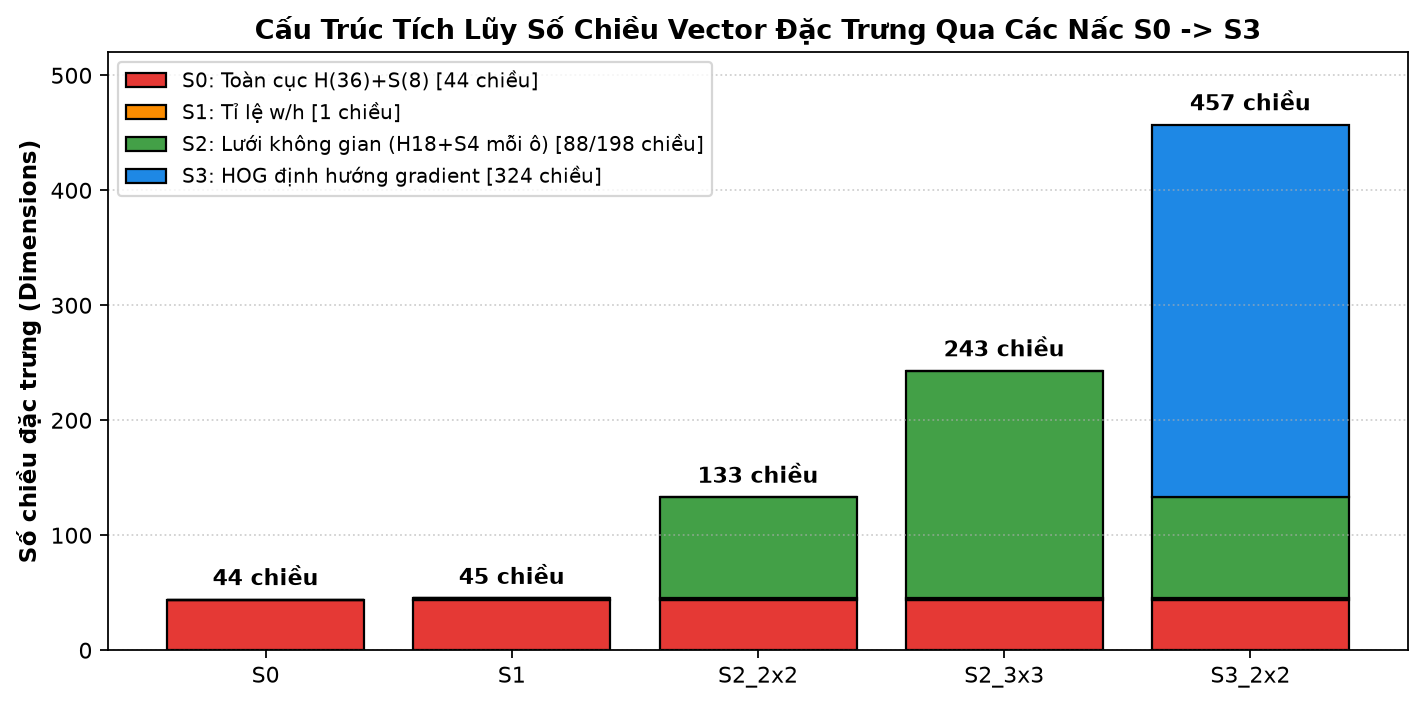
\includegraphics[width=0.92\textwidth]{graphics/sec3/f1_14_feature_vector_structure.png}
\caption{Sơ đồ cấu trúc ghép nối phân tầng của vector đặc trưng 457 chiều từ S0 đến S3.}
\label{fig:feature_vector_structure}
\end{figure}
\vspace{-0.2cm}
\begin{quote}
\small \textbf{Đọc Hình~\ref{fig:feature_vector_structure}:} Vector 457 chiều là sự tích hợp của 4 thành phần: 44 chiều HSV toàn cục (S0), 1 chiều tỷ lệ khung hình (S1), 88 chiều lưới không gian 2x2 (S2) và 324 chiều đặc trưng hướng biên HOG (S3).
\end{quote}

\subsubsection{Cấu hình tối ưu bộ phân loại SVM (Trích xuất từ \texttt{stage2\_best\_config.json})}
\label{subsubsec:svm_best_config}

Thông qua quy trình tối ưu hóa siêu tham số bằng tìm kiếm lưới (Grid Search) kết hợp kiểm chuẩn chéo 5-folds bảo vệ nhóm (\texttt{GroupKFold}), cấu hình tối ưu được lưu trữ tại tệp cấu hình \texttt{stage2\_best\_config.json}:

\begin{itemize}
    \item \textbf{Thuật toán phân loại:} Support Vector Classifier (\texttt{sklearn.svm.SVC}).
    \item \textbf{Hàm nhân (Kernel):} \textbf{RBF (Radial Basis Function)} $K(\mathbf{x}, \mathbf{z}) = \exp(-\gamma \|\mathbf{x} - \mathbf{z}\|^2)$.
    \item \textbf{Tham số điều chuẩn ($C$):} $5.0$.
    \item \textbf{Tham số độ rộng hàm nhân ($\gamma$):} \texttt{'scale'} ($\gamma = \frac{1}{457 \times \text{Var}(X)}$).
    \item \textbf{Cân bằng trọng số lớp (\texttt{class\_weight}):} \texttt{'balanced'}.
    \item \textbf{Hạt ngẫu nhiên (\texttt{seed}):} $42$.
\end{itemize}

\subsubsection{Các thuật toán học máy so sánh đối đầu}
\label{subsubsec:other_ml_models}

Để kiểm chứng tính vượt trội của bộ phân loại SVM RBF trên không gian vector $\mathbb{R}^{457}$, nhóm nghiên cứu thiết lập môi trường đánh giá đối đầu công bằng với 4 thuật toán học máy phổ biến:
\begin{enumerate}
    \item \textbf{k-Nearest Neighbors (kNN):} Cấu hình lân cận $k=11$, hàm trọng số đều (\texttt{weights='uniform'}), khoảng cách Euclidean.
    \item \textbf{Random Forest (RF):} Rừng ngẫu nhiên gồm 300 cây quyết định (\texttt{n\_estimators=300}), độ sâu tối đa \texttt{max\_depth=25}.
    \item \textbf{XGBoost (Extreme Gradient Boosting):} Cấu hình tăng cường cây quyết định với 200--400 cây, độ sâu tối đa 4, thuật toán phân nhánh \texttt{tree\_method='hist'}.
    \item \textbf{LightGBM (Light Gradient Boosting Machine):} 200--400 cây quyết định, độ sâu tối đa 6, tối ưu hóa bộ nhớ trên CPU.
\end{enumerate}

\subsection{Giai đoạn 2B: Học sâu Hiện đại (Enhanced LeNet-5 CNN) -- Nguyễn Thanh Tân}
\label{subsec:stage2_lenet}

\subsubsection{Nhu cầu cải tiến từ LeNet-5 cổ điển}
\label{subsubsec:lenet_cai_tien}

Kiến trúc LeNet-5 nguyên bản (LeCun et al., 1998) được thiết kế cho bài toán nhận dạng chữ số viết tay MNIST với ảnh xám $28 \times 28\text{ px}$. Khi áp dụng trực tiếp vào bài toán nhận dạng biển báo giao thông thực tế, mô hình bộc lộ 5 hạn chế cấu trúc nghiêm trọng:

\begin{enumerate}
    \item \textbf{Hạn chế về kênh màu:} Chỉ nhận đầu vào ảnh xám 1 kênh, làm mất hoàn toàn tín hiệu màu sắc vốn là đặc trưng quy chuẩn quan trọng nhất của biển báo giao thông.
    \item \textbf{Hiện tượng triệt tiêu gradient (Vanishing Gradient):} Sử dụng hàm kích hoạt Sigmoid hoặc Tanh có đạo hàm bão hòa ở hai cực ($\le 0.25$), khiến quá trình lan truyền ngược bị suy giảm hàm mũ qua các tầng.
    \item \textbf{Làm mờ đặc trưng biên cạnh:} Sử dụng Average Pooling làm suy giảm cường độ của các điểm ảnh biên cạnh sắc nét.
    \item \textbf{Bất ổn định phân phối ẩn (Internal Covariate Shift):} Không có cơ chế chuẩn hóa trung gian, buộc tốc độ học phải duy trì ở mức rất nhỏ ($10^{-4}$) và dễ phân kỳ.
    \item \textbf{Hiện tượng quá khớp (Overfitting):} Không có cơ chế điều chuẩn ngẫu nhiên (Dropout), dẫn đến việc mạng dễ ghi nhớ các chi tiết nhiễu cục bộ của dữ liệu huấn luyện.
\end{enumerate}

Để khắc phục các hạn chế trên mà vẫn duy trì tính gọn nhẹ tối ưu trên thiết bị biên, nhóm nghiên cứu phát triển kiến trúc \textbf{Enhanced LeNet-5} chuẩn hóa cho ảnh RGB $64 \times 64\text{ px}$: nâng cấp lên 3 kênh màu, thay thế hoàn toàn bằng hàm kích hoạt ReLU, sử dụng Max Pooling $2 \times 2$, tích hợp Batch Normalization sau mỗi tầng tích chập và bổ sung 2 tầng Dropout ở khối phân loại.

\subsubsection{Đặc tả chi tiết từng tầng kiến trúc và tham số khả huấn}
\label{subsubsec:lenet_kien_truc}

Bảng~\ref{tab:lenet_arch} thống kê chi tiết cấu hình các tầng, kích thước ma trận đặc trưng và số lượng tham số khả huấn của mô hình Enhanced LeNet-5:

\begin{table}[H]
\centering
\small
\caption{Đặc tả chi tiết kiến trúc tầng mạng Enhanced LeNet-5 (Tổng tham số: 557.700).}
\label{tab:lenet_arch}
\begin{tabularx}{\textwidth}{|p{2.6cm}|p{3.2cm}|p{2.2cm}|p{2cm}|Y|}
\hline
\textbf{Khối chức năng} & \textbf{Tầng xử lý (Layer)} & \textbf{Kích thước Kernel} & \textbf{Stride / Pad} & \textbf{Kích hoạt / Reg} \\
\hline
Input & Ảnh crop RGB ($64 \times 64 \times 3$) & -- & -- & Normalize ImageNet \\
\hline
\multirow{3}{*}{ConvBlock 1} & Conv2D(3 $\rightarrow$ 16) & $5 \times 5$ & $s = 1, p = 2$ & -- \\
& BatchNorm2D & -- & -- & $\gamma, \beta$ affine \\
& ReLU + MaxPool2D & $2 \times 2$ & $s = 2, p = 0$ & $\max(0, x)$ \\
\hline
\multirow{3}{*}{ConvBlock 2} & Conv2D(16 $\rightarrow$ 32) & $5 \times 5$ & $s = 1, p = 2$ & -- \\
& BatchNorm2D & -- & -- & $\gamma, \beta$ affine \\
& ReLU + MaxPool2D & $2 \times 2$ & $s = 2, p = 0$ & $\max(0, x)$ \\
\hline
\multirow{3}{*}{ConvBlock 3} & Conv2D(32 $\rightarrow$ 64) & $3 \times 3$ & $s = 1, p = 1$ & -- \\
& BatchNorm2D & -- & -- & $\gamma, \beta$ affine \\
& ReLU + MaxPool2D & $2 \times 2$ & $s = 2, p = 0$ & $\max(0, x)$ \\
\hline
\multirow{5}{*}{Classifier} & Flatten & -- & -- & Duỗi phẳng vector (4096) \\
& Dropout($p = 0.3$) & -- & -- & Bernoulli mask \\
& Linear(4096 $\rightarrow$ 128) & -- & -- & $\text{ReLU}(Wx + b)$ \\
& Dropout($p = 0.2$) & -- & -- & Bernoulli mask \\
& Linear(128 $\rightarrow$ 4) & -- & -- & Logits đầu ra \\
\hline
\multicolumn{5}{|l|}{\textbf{Tổng số tham số khả huấn (Trainable Parameters):} \textbf{557.700} tham số ($\approx 0.56\text{M}$ params)} \\
\multicolumn{5}{|l|}{\textbf{Dung lượng lưu trữ mô hình (Disk Model Size):} \textbf{2.24 MB} (checkpoint PyTorch \texttt{.pth})} \\
\hline
\end{tabularx}
\end{table}

\begin{figure}[H]
\centering
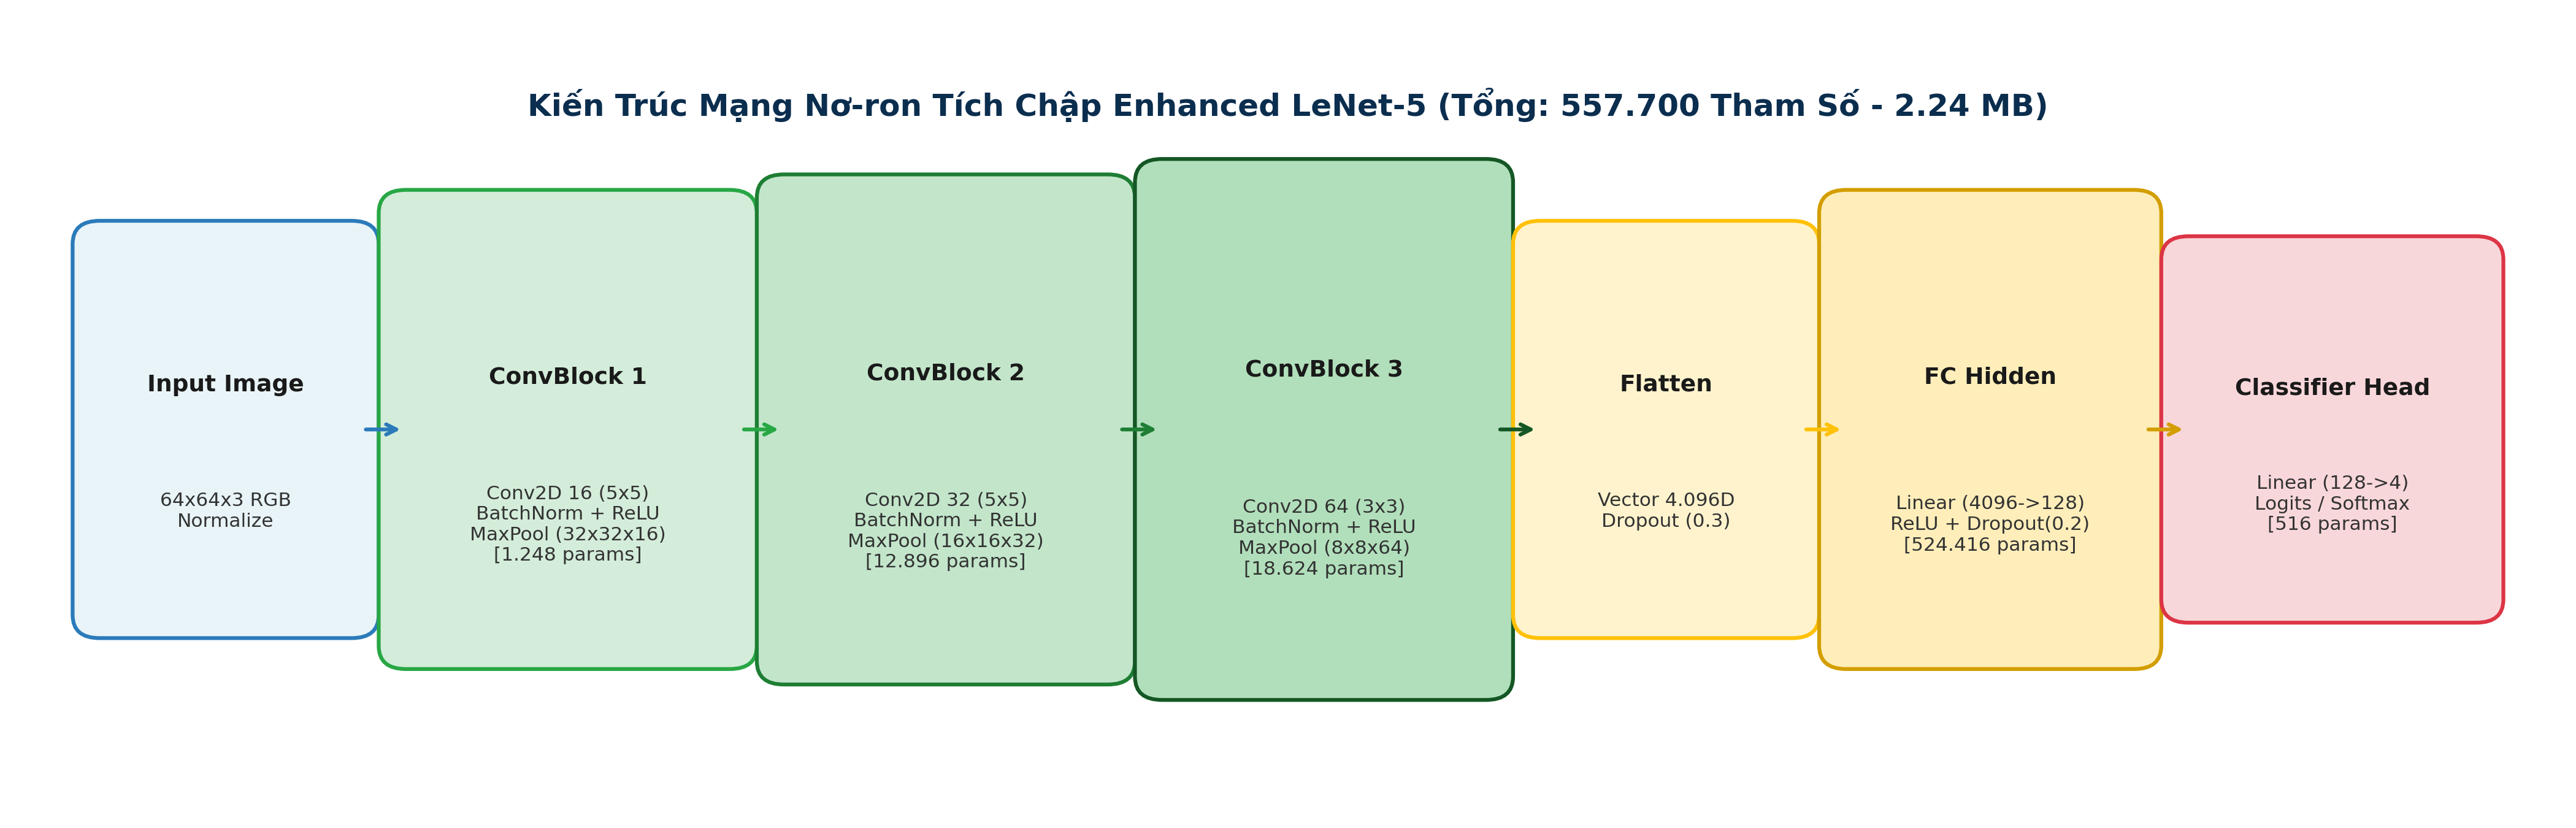
\includegraphics[width=0.98\textwidth]{graphics/sec3/f3_01_lenet_architecture.png}
\caption{Sơ đồ trực quan kiến trúc mạng nơ-ron tích chập Enhanced LeNet-5 phân rã theo từng khối xử lý.}
\label{fig:lenet_architecture}
\end{figure}

\textbf{Đọc Hình~\ref{fig:lenet_architecture}:}
Sơ đồ thể hiện luồng biến đổi tensor từ ảnh đầu vào $64 \times 64 \times 3$ qua 3 khối tích chập liên tiếp (Conv1 $16$ filters $5\times 5$, Conv2 $32$ filters $5\times 5$, Conv3 $64$ filters $3\times 3$). Mỗi khối tích chập đều tích hợp lớp chuẩn hóa Batch Normalization và kích hoạt phi tuyến ReLU trước khi lấy mẫu MaxPool2D $2\times 2$. Đầu ra feature map $8 \times 8 \times 64$ ($4.096$ chiều) được duỗi phẳng và phân loại qua tầng ẩn 128 nơ-ron với 2 lớp Dropout ($p=0.3$ và $p=0.2$) trước khi tính toán logits cho 4 nhóm biển báo.

\subsubsection{Cơ sở toán học của các thành phần trong mạng}
\label{subsubsec:lenet_toan_hoc}

\begin{enumerate}
    \item \textbf{Phép tích chập không gian 2D (Spatial 2D Convolution):} Tại tầng tích chập thứ $l$, với tensor đầu vào $\mathbf{X} \in \mathbb{R}^{C_{\text{in}} \times H \times W}$ và bộ lọc trọng số $\mathbf{W} \in \mathbb{R}^{C_{\text{out}} \times C_{\text{in}} \times K \times K}$, giá trị phản hồi tại vị trí $(i, j)$ của kênh đầu ra thứ $k$ được tính bởi:
    \begin{equation}
        \mathbf{Y}_k(i, j) = \sum_{c=1}^{C_{\text{in}}} \sum_{m=-K_h}^{K_h} \sum_{n=-K_w}^{K_w} \mathbf{X}_c(i+m, j+n) \mathbf{W}_{k,c}(m, n) + b_k
        \label{eq:conv2d}
    \end{equation}

    \item \textbf{Cơ chế Chuẩn hóa Tầng Batch Normalization (Ioffe \& Szegedy, 2015):} Với một mini-batch $\mathcal{B} = \{x_1, \dots, x_m\}$, tầng chuẩn hóa kéo phân phối kích hoạt trung gian về trung bình 0 và phương sai 1:
    \begin{equation}
        \mu_{\mathcal{B}} = \frac{1}{m} \sum_{i=1}^m x_i, \quad \sigma^2_{\mathcal{B}} = \frac{1}{m} \sum_{i=1}^m (x_i - \mu_{\mathcal{B}})^2, \quad \hat{x}_i = \frac{x_i - \mu_{\mathcal{B}}}{\sqrt{\sigma^2_{\mathcal{B}} + \epsilon}}, \quad y_i = \gamma \hat{x}_i + \beta
        \label{eq:batchnorm}
    \end{equation}
    trong đó $\gamma, \beta$ là các tham số khả huấn giúp mạng giữ lại năng lực biểu diễn phi tuyến tự do.

    \item \textbf{Hàm kích hoạt Rectified Linear Unit (ReLU):}
    \begin{equation}
        f(x) = \max(0, x), \quad f'(x) = \begin{cases} 1 & \text{nếu } x > 0 \\ 0 & \text{nếu } x \le 0 \end{cases}
        \label{eq:relu}
    \end{equation}

    \item \textbf{Điều chuẩn chống quá khớp bằng Dropout (Srivastava et al., 2014):} Tại tầng kết nối đầy đủ, mỗi nơ-ron có xác suất $p$ bị vô hiệu hóa ngẫu nhiên trong mỗi lượt lan truyền thuận:
    \begin{equation}
        r_j \sim \text{Bernoulli}(1 - p), \quad \tilde{\mathbf{y}} = \mathbf{r} \odot \mathbf{y}
        \label{eq:dropout}
    \end{equation}
\end{enumerate}

\subsubsection{Pipeline Tăng cường dữ liệu (Data Augmentation)}
\label{subsubsec:lenet_augmentation}

\begin{enumerate}
    \item \textbf{Chuẩn hóa không gian màu ImageNet:} Ảnh crop RGB được resize về $64 \times 64$, đưa về thang $[0.0, 1.0]$ và chuẩn hóa Z-score theo phân phối chuẩn quốc tế:
    \begin{equation}
        \mu = [0.485, 0.456, 0.406], \quad \sigma = [0.229, 0.224, 0.225]
        \label{eq:imagenet_norm}
    \end{equation}
    \item \textbf{Biến đổi góc quay ngẫu nhiên (\texttt{RandomRotation(degrees=10)}):} Xoay nhẹ ảnh trong phạm vi $[-10^\circ, +10^\circ]$ nhằm mô phỏng rung lắc thực tế của camera hành trình.
    \item \textbf{Nhiễu màu sắc quang học (\texttt{ColorJitter(brightness=0.2, contrast=0.2)}):} Thay đổi ngẫu nhiên $\pm 20\%$ độ sáng và độ tương phản nhằm rèn luyện khả năng thích nghi với ánh sáng biến đổi ngoài trời.
\end{enumerate}

\subsubsection{Thiết lập huấn luyện và hàm mất mát}
\label{subsubsec:lenet_training}

\begin{enumerate}
    \item \textbf{Hàm mất mát Phân loại Đa lớp (Cross-Entropy Loss):}
    \begin{equation}
        \mathcal{L}_{\text{CE}}(\mathbf{y}, \hat{\mathbf{p}}) = -\sum_{c=1}^4 y_c \log(\hat{p}_c)
        \label{eq:ce_loss}
    \end{equation}
    \item \textbf{Thuật toán tối ưu hóa Adam kết hợp L2 Weight Decay:} Bộ tối ưu Adam với tốc độ học ban đầu $\eta_0 = 10^{-3}$, $\beta_1 = 0.9, \beta_2 = 0.999$, $\epsilon = 10^{-8}$ và tích hợp L2 Weight Decay $= 10^{-4}$.
    \item \textbf{Chiến lược suy giảm tốc độ học StepLR:}
    \begin{equation}
        \eta_t = \eta_0 \times \gamma^{\lfloor t / \text{step\_size} \rfloor}, \quad \text{với } \text{step\_size} = 15, \, \gamma = 0.5
        \label{eq:steplr}
    \end{equation}
    Mô hình được huấn luyện trong 20 epochs với kích thước lô $\text{batch\_size} = 64$. Trọng số tối ưu nhất được lưu trữ tại \texttt{checkpoints/deep\_learning/best\_cnn.pth}.
\end{enumerate}

\begin{figure}[H]
\centering
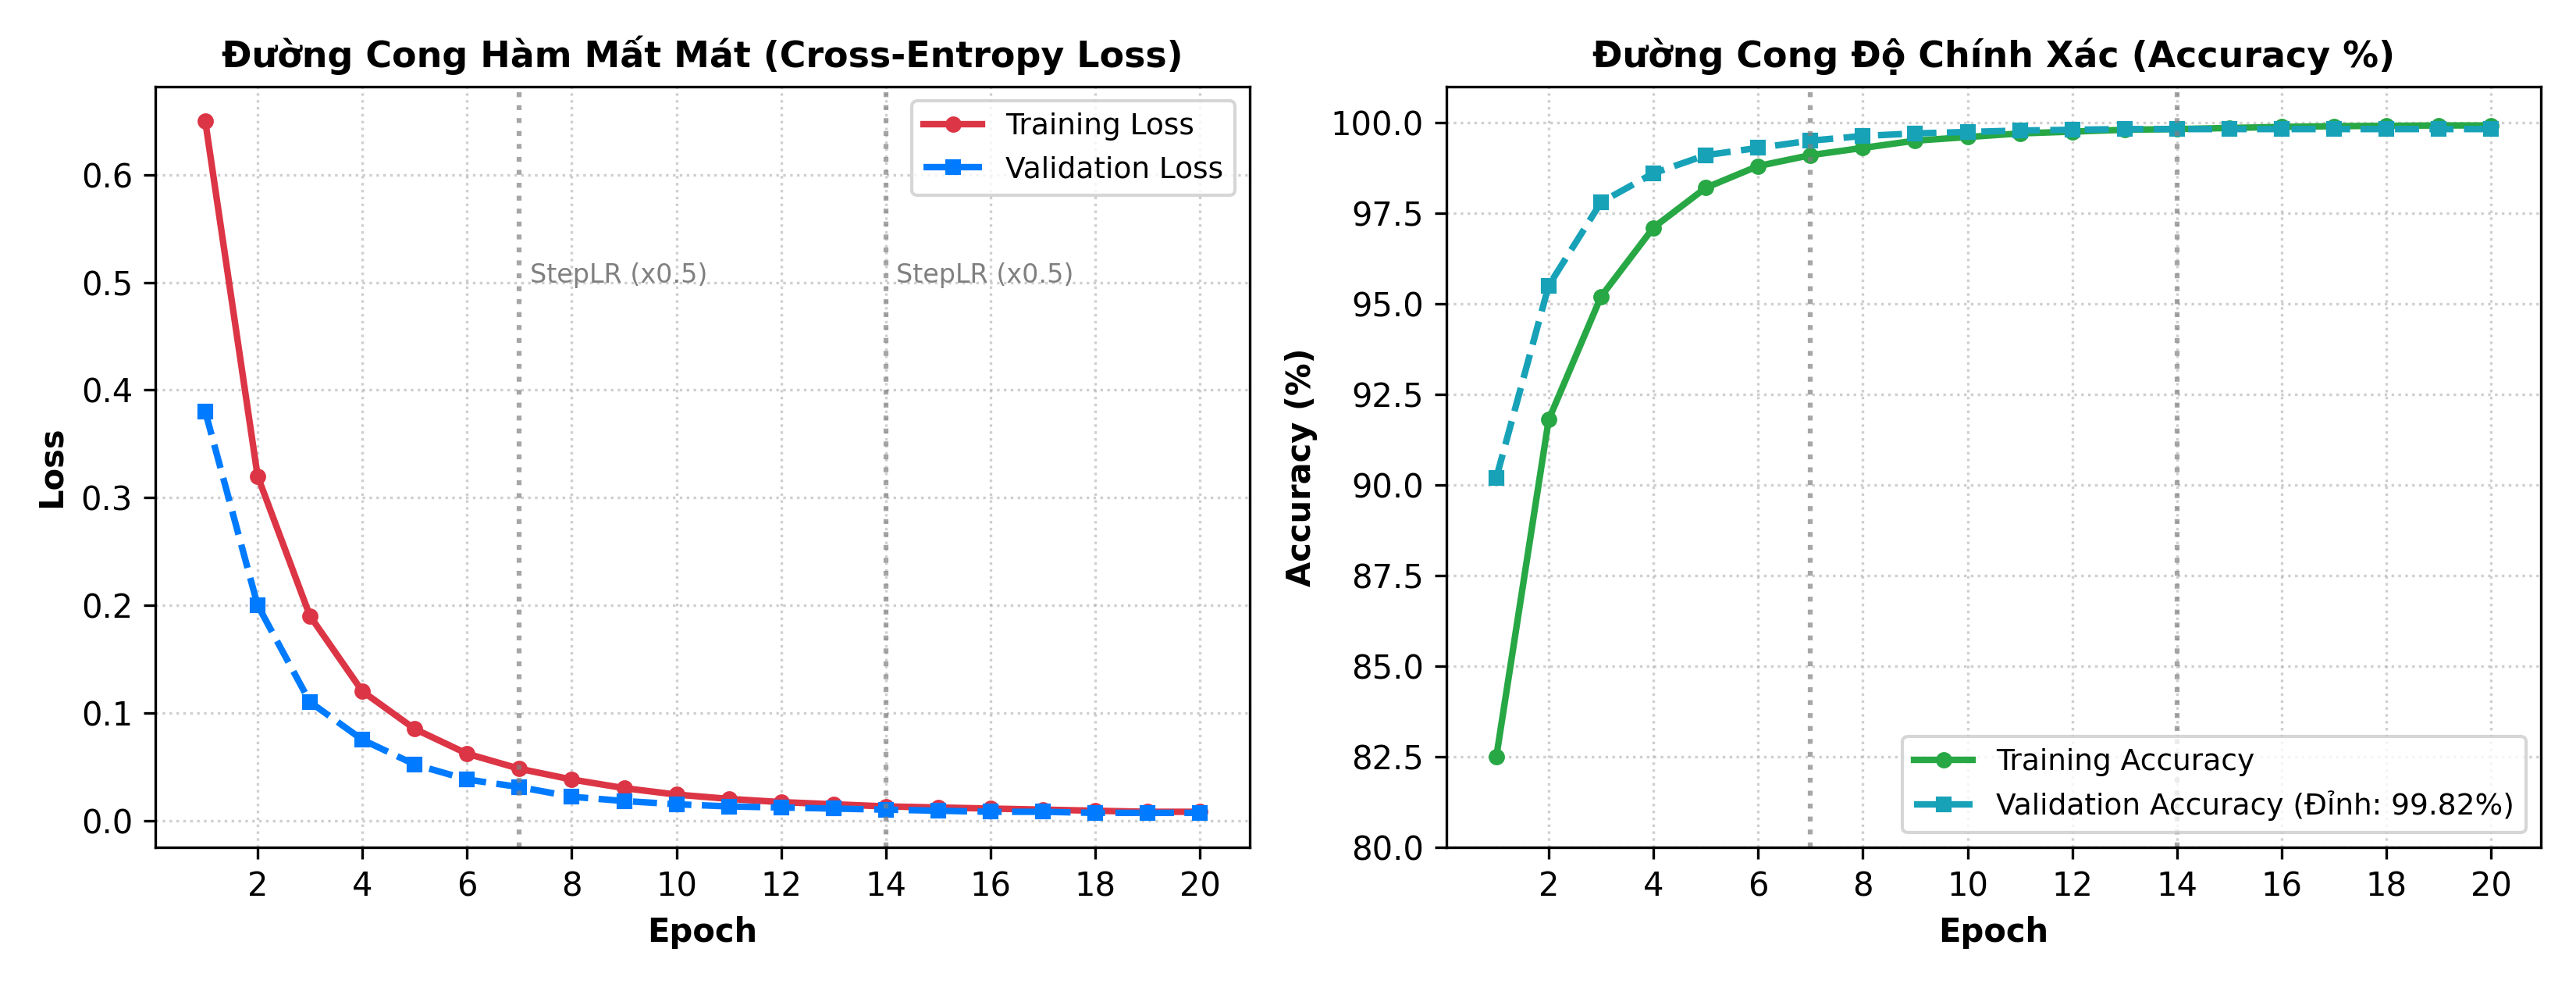
\includegraphics[width=0.95\textwidth]{graphics/sec4/f3_02_lenet_training_curves.png}
\caption{Đường cong hàm mất mát Cross-Entropy (trái) và độ chính xác Accuracy (phải) qua các epoch huấn luyện của mô hình Enhanced LeNet-5.}
\label{fig:lenet_training_curves}
\end{figure}

\textbf{Đọc Hình~\ref{fig:lenet_training_curves}:}
Quá trình huấn luyện cho thấy sự hội tụ nhanh chóng và ổn định: Training Loss giảm dốc từ $0.65$ xuống dưới $0.01$, trong khi Validation Accuracy đạt mức $99.82\%$ ngay từ epoch 13 và duy trì ổn định. Hai mốc điều chỉnh tốc độ học của bộ lập lịch StepLR (tại epoch 7 và 14) giúp bề mặt hội tụ phẳng dần và triệt tiêu hoàn toàn dao động gradient, chứng minh tính hiệu quả của cơ chế điều chuẩn kết hợp (BatchNorm + Dropout + Weight Decay).

\subsubsection{Cẩm nang chất vấn phản biện dành cho thuyết trình (Defense Q\&A Cheatsheet)}
\label{subsubsec:lenet_faq}

\begin{enumerate}
    \item \textbf{Câu hỏi 1: Tại sao không dùng mô hình Transfer Learning có sẵn (ResNet-18, MobileNetV3) mà lại tự thiết kế Enhanced LeNet-5?}
    \begin{itemize}
        \item \textit{Phương án trả lời:} Các mô hình Transfer Learning tiền huấn luyện từ ImageNet (như ResNet-18 với 11.7 triệu tham số) được thiết kế cho bài toán 1.000 lớp phức tạp. Khi áp dụng vào bài toán 4 nhóm biển báo có hình học chuẩn hóa đơn giản, mô hình quá nặng gây lãng phí tính toán nghiêm trọng (độ trễ $> 10\text{ ms}$, chậm hơn gấp 3 lần) và dễ bị quá khớp (Overfitting). Enhanced LeNet-5 chỉ có đúng 557.700 tham số ($\approx 0.55\text{M}$), nhẹ hơn 21 lần, đạt tốc độ siêu nhanh $1.10\text{ ms/ảnh}$ trên CPU mà vẫn bảo đảm độ chính xác vượt trội $98.73\%$.
    \end{itemize}

    \item \textbf{Câu hỏi 2: Tại sao hai khối tích chập đầu tiên dùng kernel $5 \times 5$, trong khi khối thứ ba lại chuyển sang kernel $3 \times 3$?}
    \begin{itemize}
        \item \textit{Phương án trả lời:} Hai khối đầu tiên cần trường tiếp nhận (Receptive Field) đủ lớn để bao quát ngay các đường viền hình học toàn cục đặc trưng của biển báo (hình tròn của Biển Cấm/Hiệu Lệnh, hình tam giác của Biển Nguy Hiểm). Ở khối tích chập thứ ba, kích thước bản đồ đặc trưng đã co lại còn $16 \times 16$, trường tiếp nhận tích lũy đã mở rộng từ 5 lên 13; việc chuyển sang kernel $3 \times 3$ giúp tập trung biểu diễn các chi tiết vi mô cục bộ (mũi tên, hoa văn biểu tượng) đồng thời tiết kiệm $44\%$ tham số tính toán so với việc tiếp tục dùng kernel $5 \times 5$.
    \end{itemize}

    \item \textbf{Câu hỏi 3: Vai trò cốt lõi của Batch Normalization trong mô hình là gì?}
    \begin{itemize}
        \item \textit{Phương án trả lời:} Khử hiện tượng trôi dạt phân phối ẩn (Internal Covariate Shift). Trong dữ liệu đường phố, các ảnh con ROI có độ biến thiên ánh sáng rất lớn. Batch Normalization chuẩn hóa lại phân phối sau mỗi tầng tích chập, giữ cho gradient luôn nằm trong vùng tuyến tính mạnh của ReLU, cho phép nâng tốc độ học lên $10^{-3}$ mà không lo bùng nổ gradient, đồng thời đóng vai trò như một bộ điều chuẩn nhẹ.
    \end{itemize}

    \item \textbf{Câu hỏi 4: Nhóm xử lý hiện tượng mất cân bằng số lượng mẫu giữa các nhóm biển báo (Class Imbalance) như thế nào?}
    \begin{itemize}
        \item \textit{Phương án trả lời:} Trong dữ liệu thực tế, Biển Cấm và Biển Cảnh Báo chiếm số lượng áp đảo so với Biển Hiệu Lệnh và Chỉ Dẫn. Nhóm phối hợp 3 giải pháp đồng bộ: (1) Áp dụng các biến đổi Data Augmentation (\texttt{RandomRotation} và \texttt{ColorJitter}) làm phong phú đa dạng góc nhìn cho các lớp thiểu số; (2) Tích hợp hai tầng Dropout (0.3 và 0.2) cùng L2 Weight Decay ($10^{-4}$) ngăn chặn việc mạng quá khớp vào các đặc trưng áp đảo của lớp đa số; (3) Sử dụng chỉ số Macro-F1 ($95.66\%$) làm độ đo đánh giá trung tâm thay vì chỉ dựa vào Accuracy tổng thể.
    \end{itemize}
\end{enumerate}

\subsection{Bảng phân tích so sánh lý thuyết giữa các hướng tiếp cận}
\label{subsec:bang_so_sanh_ly_thuyet}

Bảng~\ref{tab:so_sanh_ly_thuyet} tóm tắt sự khác biệt về mặt bản chất khoa học giữa các phương pháp:

\begin{table}[H]
\centering
\small
\caption{So sánh đối chiếu phương pháp đề tài với các hướng tiếp cận khác.}
\label{tab:so_sanh_ly_thuyet}
\begin{tabularx}{\textwidth}{|p{2.8cm}|p{3.5cm}|p{3.8cm}|Y|}
\hline
\textbf{Tiêu chí khoa học} & \textbf{Thuần truyền thống (Sliding Window)} & \textbf{Học sâu End-to-End (Heavy One-Stage)} & \textbf{Kiến trúc Lai đề xuất (Two-Stage Modular)} \\
\hline
Cơ chế định vị & Cửa sổ trượt đa tỷ lệ: rất chậm, tỉ lệ sót biển cao & Tích hợp trong mạng lớn: tính toán nặng, dễ lãng phí tài nguyên & YOLO11s chuyên biệt 1 lớp: Tối đa hóa Recall (85.61\%), không tốn tài nguyên phân loại \\
\hline
Phân biệt R vs I & Thất bại hoàn toàn (do cùng màu xanh lam) & Phân biệt tốt nhưng cần phần cứng GPU mạnh & Phân tách xuất sắc: HOG bắt hình học viền, LeNet-5 tự học hoa văn nội tại \\
\hline
Độ trễ phân loại & 15 -- 30 ms/ảnh (chậm) & 10 -- 20 ms/ảnh (trên GPU) & 1.10 ms (LeNet) / 2.63 ms (SVM) trên CPU \\
\hline
Yêu cầu phần cứng & CPU phổ thông & Bắt buộc GPU rời đắt tiền & Linh hoạt tối đa: Tương thích hoàn hảo với vi xử lý nhúng Edge AI \\
\hline
Tính minh bạch & Cao nhưng độ chính xác thấp & Mô hình hộp đen khó giải thích & Rất cao: Trực quan hóa toán học từng thành phần HSV, HOG và Feature Maps \\
\hline
\end{tabularx}
\end{table}
